% Peekaboo-VL report: 03_data. Included from ../peekaboo_report.tex.
\section{Task and Data}
\label{sec:data}

\subsection{The benchmark}
Each ReVA record has a video path, a question, four options (A--D) and, for
training data, the correct letter. The questions fall into eleven tasks in
four groups (Table~\ref{tab:tasks}). The challenge test set has 4,000
questions over 1,014 clips. The score is accuracy, overall and per task.
Fig.~\ref{fig:sample} shows one training clip with three of its questions,
and Fig.~\ref{fig:gallery} shows one question from each video source.

\begin{figure*}[t]
\centering
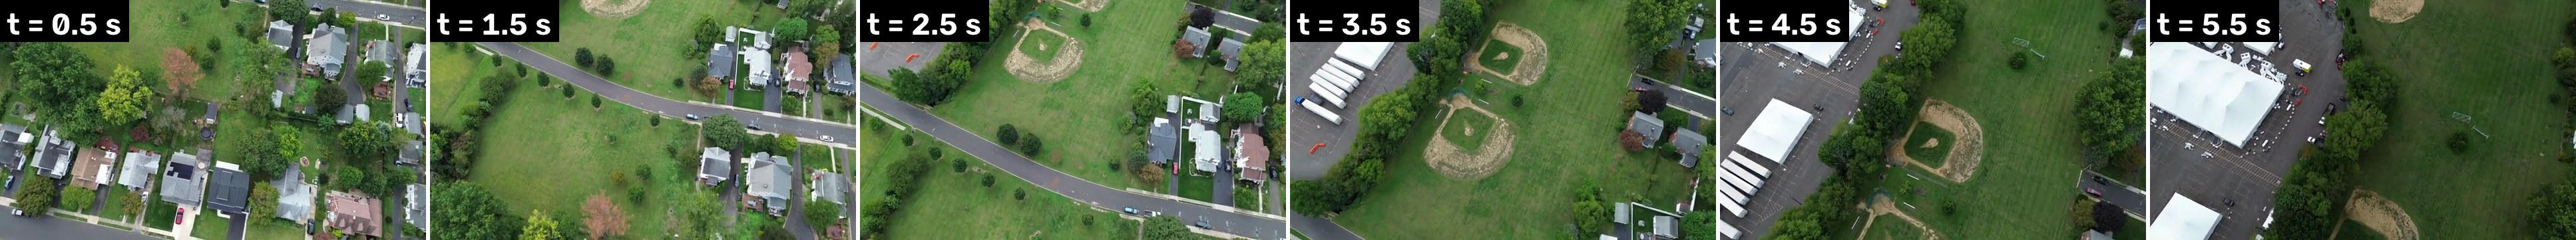
\includegraphics[width=\textwidth]{figures/sample_frames.jpg}\\[3pt]
\footnotesize
\begin{tabular}{@{}p{0.11\textwidth}p{0.42\textwidth}p{0.40\textwidth}@{}}
\toprule
Task & Question & Options (correct one in bold) \\
\midrule
TU\_Temporal & At what point in the video do the white tents first appear in the frame? &
A.~4.8\,s \quad \textbf{B.~3.5\,s} \quad C.~2.0\,s \quad D.~0.0\,s \\
SR\_Viewpoint & What is the primary camera motion state throughout the video? &
A.~Panning left/right \quad \textbf{B.~Moving forward} \quad C.~Zooming in/out \quad D.~Rotating \\
FP\_Change & How does the camera's perspective change throughout the video? &
\textbf{D.~From a wide aerial view of the neighborhood to a closer view of the field and tents} (3 other options) \\
\midrule
\multicolumn{3}{@{}l@{}}{\textit{Our motion hint for this clip:} ``Camera motion: 0.1--5.9s moving
forward quickly while rotating clockwise. Mostly moving forward (100\% of the clip).''} \\
\bottomrule
\end{tabular}
\caption{A ReVA training clip (\texttt{Hawk\_UAV/PH/DJI\_0229\_d4\_01}):
six evenly spaced frames with their true times, three of its questions, and
the motion hint our system writes for it. The tents enter the frame at
$t{=}3.5$\,s, which is the answer to the temporal question. The hint
already contains the answer to the camera-motion question, in the option's
own words.}
\label{fig:sample}
\end{figure*}


\begin{figure*}[t]
\centering
\footnotesize
\setlength{\tabcolsep}{3pt}
\resizebox{\textwidth}{!}{%
\begin{tabular}{@{}c@{\hspace{6pt}}c@{}}
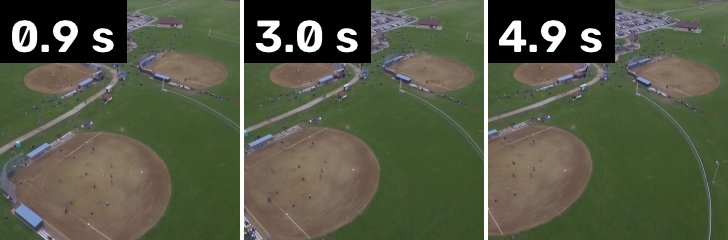
\includegraphics[height=19mm]{figures/gallery_era.jpg} &
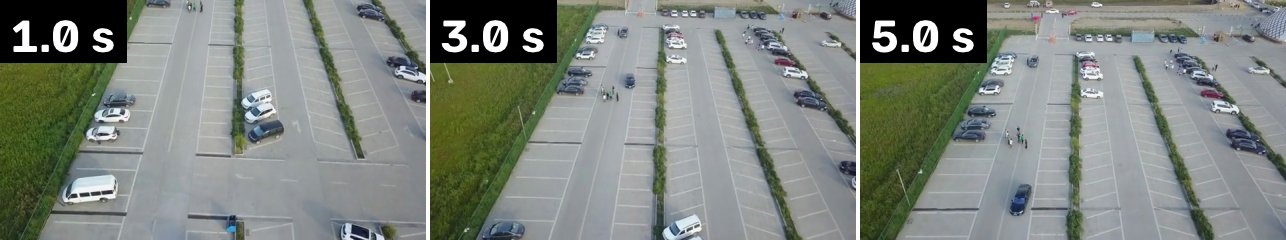
\includegraphics[height=19mm]{figures/gallery_visdrone.jpg} \\[1pt]
\parbox[t]{0.31\textwidth}{\textbf{ERA, CR\_Causation.} Likely cause of the many parked cars?
\textbf{(B) Baseball games} (vs.\ restaurant, highway, mall).} &
\parbox[t]{0.55\textwidth}{\textbf{VisDrone, FP\_ObjectLand.} What type of land cover is visible on
the left side of the parking lot? (A) A paved road \ (B) A body of water \ (C) A dense forest \
\textbf{(D) A field of green grass}.} \\[20pt]
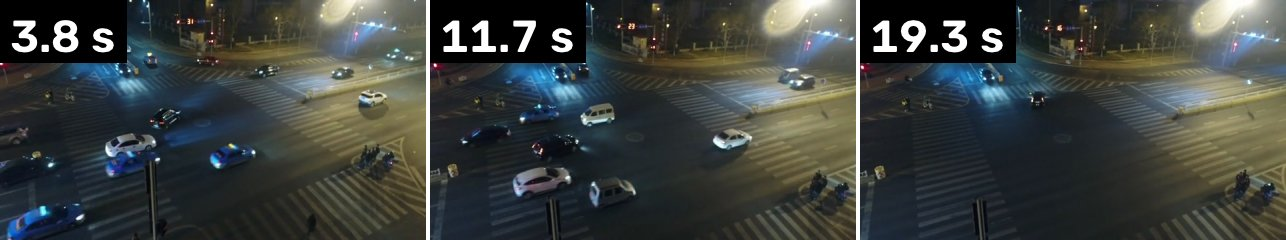
\includegraphics[height=16mm]{figures/gallery_uavdt.jpg} &
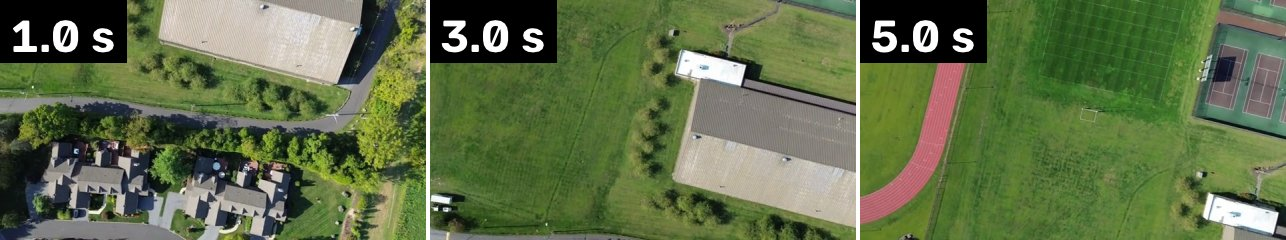
\includegraphics[height=16mm]{figures/gallery_hawk.jpg} \\[1pt]
\parbox[t]{0.46\textwidth}{\textbf{UAVDT, TU\_Temporal} (23.2\,s clip). At what time does the white
van first appear in the video? (A) 0:08 \ (B) 0:12 \ \textbf{(C) 0:03} \ (D) 0:05.} &
\parbox[t]{0.46\textwidth}{\textbf{Hawk-UAV, SR\_Geometric.} How is the tennis court positioned
relative to the soccer field? (A) Above \ (B) To the left \ (C) Below \ \textbf{(D) To the right}.} \\
\end{tabular}}
\caption{One example from each of the four video sources, three evenly spaced frames each with
their true times (correct answers in bold). ERA clips are square and about 6\,s long; UAVDT clips
can last tens of seconds; temporal questions use both seconds and \texttt{m:ss} formats.}
\label{fig:gallery}
\end{figure*}

\begin{table}[t]
\centering
\caption{The eleven tasks and how many test questions each has.}
\label{tab:tasks}
\footnotesize
\begin{tabular}{@{}llr@{}}
\toprule
Group & Task (leaderboard name) & Test Q \\
\midrule
\multirow{3}{*}{Factual Perception} & General Understanding (FP\_General) & 180 \\
 & Object \& Land Cover (FP\_ObjectLand) & 660 \\
 & Change Detection (FP\_Change) & 500 \\
\midrule
\multirow{2}{*}{Temporal} & Temporal Grounding (TU\_Temporal) & 640 \\
 & Trend \& Pattern (TU\_TrendPattern) & 360 \\
\midrule
\multirow{3}{*}{Spatial} & Geometric Relation (SR\_Geometric) & 400 \\
 & Structural Layout (SR\_Structural) & 340 \\
 & Perspective \& Viewpoint (SR\_Viewpoint) & 480 \\
\midrule
\multirow{3}{*}{Causal} & Causation (CR\_Causation) & 180 \\
 & Consequence (CR\_Consequence) & 100 \\
 & Hypothetical (CR\_Hypothetical) & 160 \\
\bottomrule
\end{tabular}
\end{table}

\textbf{What the tasks ask, in plain words.}
\emph{General Understanding} asks what the video is about or what is in it.
\emph{Object \& Land Cover} asks what kinds of objects or ground (grass,
water, buildings) appear, and sometimes how many. \emph{Change Detection}
asks how something changes during the clip, such as how a car moves or how
the view changes. \emph{Temporal Grounding} asks when something happens, as
a time or a time range. \emph{Trend \& Pattern} asks about repeated or
overall movement, such as the main direction of traffic. The three spatial
tasks ask where things are relative to each other, how the area is laid
out (for example, a grid of roads), and how the camera looks at or moves
over the scene. The three causal tasks ask why something happens, what will
happen next, and what would happen if something were different. These last
three rely mostly on general knowledge and are already easy for large
models.

\subsection{What the data files reveal: same videos, new questions}
Before building anything, we checked the released files carefully.
Table~\ref{tab:audit} summarizes what we found.

The most important fact is this: 1,012 of the 1,014 test clips, and all 529
longer source videos they were cut from, also appear in the training set.
3,997 of the 4,000 test questions are about a clip that has training
questions. But the test questions themselves are new. Only 24 are exact
copies of a training question on the same clip, and 334 are close copies
(at least 60\% of their words in common). So the test asks \emph{new
questions about videos the model has already seen in training}.

The official validation set is different. 1,572 of its 2,000 questions
repeat a training question on the same clip, and 1,569 of those have the
same answer. A model trained on the training set will look good on
this validation set simply because it remembers the answers. That number
would tell us little about the test.

\begin{table}[t]
\centering
\caption{What the released annotation files show.}
\label{tab:audit}
\footnotesize
\begin{tabular}{@{}lr@{}}
\toprule
Statistic & Value \\
\midrule
Train / val / test questions & 15,773 / 2,000 / 4,000 \\
Train / val / test clips & 1,045 / 379 / 1,014 \\
Test clips also in train & 1,012 / 1,014 \\
Test questions on train clips & 3,997 / 4,000 \\
Test exact copies of train questions & 24 \\
Test close copies (word overlap $\geq 0.6$ / $\geq 0.8$) & 334 / 67 \\
Val exact copies of train questions & 1,572 / 2,000 \\
Correct answer is the longest option (train+val) & 36.3\% \\
\midrule
Our fit / dev split (questions) & 14,068 / 2,078 \\
Dev questions on fit clips & 2,074 / 2,078 \\
\bottomrule
\end{tabular}
\end{table}

\subsection{A development split that behaves like the test}
Because the official validation set cannot be trusted, we built our own
split. Our \emph{dev} set has two parts: the 428 validation questions that
are \emph{not} copies of training questions, and 150 randomly chosen
training questions per task, set aside. Our \emph{fit} set (the data we
train on) is everything else, after removing every record that asks a dev
question about the same clip. The clips are still shared between fit and
dev, just as they are shared between train and test. This copies the
``same video, new question'' setting of the real test.

One property of this split must be stated plainly. The 428 validation
questions that are not copies of training questions turn out to be copies
of \emph{test} questions: all 428 have the same clip and the same question
text as a test question. So 20.6\% of dev are test questions whose answers
the official validation file contains. They are not training answers, so
dev has no training-answer leak, but dev is not disjoint from the test,
and its agreement with the test score is partly built in. The other 1,650
dev questions are held-out training questions.

The dev set has 2,078 questions. With that many questions, the accuracy has
a margin of error of about $\pm 0.9$ points. Dev tracks the test well: our
blind scorer gets 55.5\% on dev and 55.9\% on the test leaderboard, and the
test-weighted dev accuracy (below) lands within 0.2 points of the test for
our first fine-tuned model and within about 1.2 points for the final one
(Sec.~\ref{sec:results}).

One more detail matters. The tasks do not have the same share of questions
in dev and in test. Dev has 150--231 questions per task, while the test has
100 to 660. Some tasks that are common in the test, such as Temporal
Grounding (640 questions), are among the hardest. So we also compute a
\emph{test-weighted} dev accuracy, where each task's dev accuracy is
weighted by its number of test questions. This is the number we use to
pick between systems.

\subsection{The clips are not all alike}
The dataset card describes 15-second clips at 640$\times$360 pixels.
Decoding all 1,047 clips used by the questions shows a different picture
(Table~\ref{tab:clips}). ERA clips are square and under 6\,s. Hawk-UAV
clips range from 0.1 to 40\,s. Ten clips are shorter than one second, yet
they carry 137 questions between them; those questions cannot be answered
from the video. Because we always show the model the same number of frames
(16 in our first runs, 32 in the final model), the time between two frames
ranges from a fraction of a second to more than two seconds. This is why the model must be told the \emph{true} time of each
frame, computed from each clip's own frame rate.

\begin{table}[t]
\centering
\caption{Clips used by the questions, by source (decoded from the released files).}
\label{tab:clips}
\footnotesize
\begin{tabular}{@{}lrcrc@{}}
\toprule
Source & Clips & Res. & fps & Length (s) min/med/max \\
\midrule
Hawk-UAV & 556 & 640$\times$360 & 30 & 0.1 / 8.0 / 40.2 \\
ERA~\cite{mou2020era} & 261 & 640$\times$640 & $\sim$24 & 5.4 / 5.8 / 5.8 \\
VisDrone~\cite{zhu2021visdrone} & 183 & 640$\times$360 & 30 & 0.2 / 6.0 / 6.0 \\
UAVDT~\cite{du2018uavdt} & 47 & 640$\times$360 & 30 & 3.9 / 16.0 / 35.0 \\
\bottomrule
\end{tabular}
\end{table}

\subsection{Training data balance}
The task mix of the training data differs from the test. Temporal
Grounding and Object \& Land Cover are 12.2\% and 11.1\% of our fit set,
but 16.0\% and 16.5\% of the test. Both are weak tasks for our model. This
suggests giving these tasks more weight during training, which is one of
the next experiments.
